\subsection{Life cycle of a Sieve module}

Upon launch, Launcher parses the command line. It decides that a Sieve must
be started. This will read the parameters stored in Psyclone. The available parameter names are:

\begin{itemize}
 \item[QueryString.Content] Regular expression for matching the content and title of a story.
 \item[QueryString.Author] Regular expression for matching the author of a story.
 \item[Topic] The topic the module is analysing for.
\end{itemize}

The Sieve will then go into its waiting loop, expecting stories on the
whiteboard. When a message comes in, an analysis is carried out, a report is
created and sent to the analysis whiteboard.

\begin{figure}[htp]
  \centering
  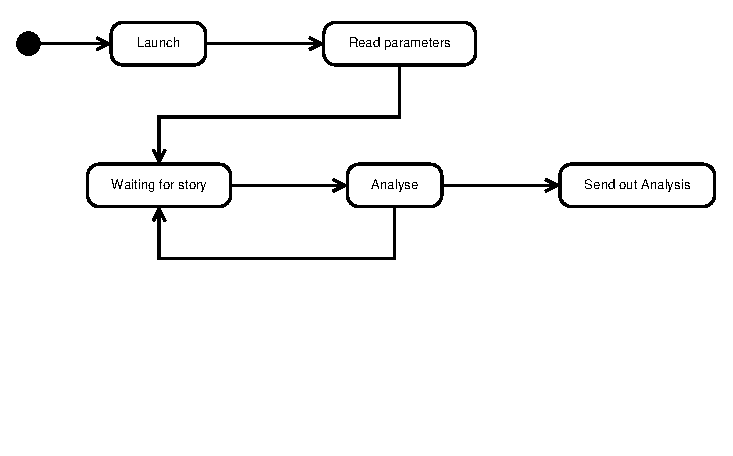
\includegraphics{design/image/sequence-diagram-sieve}
  \caption{Sequence diagram of a Sieve module}
\end{figure}
